\chapter{Fundamento teórico} \label{chap:teoria}

En este primer capítulo se explican los fundamentos teóricos necesarios para poder desarrollar e interpretar las simulaciones del resto del trabajo. Antes de entrar en el método Montecarlo y los algoritmos usados, conviene precisar el sistema de estudio y con qué magnitudes se describe. Partiendo del origen físico del ferromagnetismo y de la transición de fase ferromagnética-paramagnética, se formaliza el modelo de Ising y su hamiltoniano, se introducen los observables relevantes y, para terminar, repasamos los conceptos (exponentes críticos, escalado de tamaño finito, tiempo de correlación), sobre los que se sustenta el análisis de los resultados obtenidos.

Un sistema ferromagnético se define por el ordenamiento en una misma dirección y sentido de los espines que lo conforman, dando así una magnetización macroscópica no nula al sumarse todas las contribuciones. Este ordenamiento se ve roto por la energía térmica del sistema: cuando esta no es suficiente para desordenar los espines, estos son capaces de mantenerse orientados, y cuando sí lo es, dejan de estarlo. De aquí surge de manera natural el concepto de temperatura crítica, que marca el punto en el que ocurre la transición de fase en función de la energía térmica del sistema. Esta transición ocurre idealmente de manera abrupta y a una temperatura finita exacta, pero debido al tamaño limitado de nuestro sistema esto no se observa así, sino que cuanto mayor es el tamaño más se aproxima al salto ideal.

Un sistema real tiene un número altísimo de componentes, y lo vamos a tratar como si estuviese en contacto con un foco térmico que varía su temperatura de manera infinitamente lenta, por lo que resulta natural describirlo mediante la colectividad canónica de la física estadística. En esta sección se revisa una descripción general de la colectividad canónica, y se derivan las expresiones necesarias para calcular los observables físicos relevantes para el sistema en estudio. Además, se define formalmente el modelo de Ising, su hamiltoniano, las aproximaciones tomadas, las condiciones de contorno utilizadas y los algoritmos implementados para su estudio.

\section{Modelo de Ising}

Procedemos con una definición completa del modelo de Ising. Este consiste en una red bidimensional cuadrada de puntos equiespaciados, en cada uno de los cuales se sitúa un espín que puede tomar dos valores discretos: $+1$ o $-1$. 
\begin{figure}
    \centering
    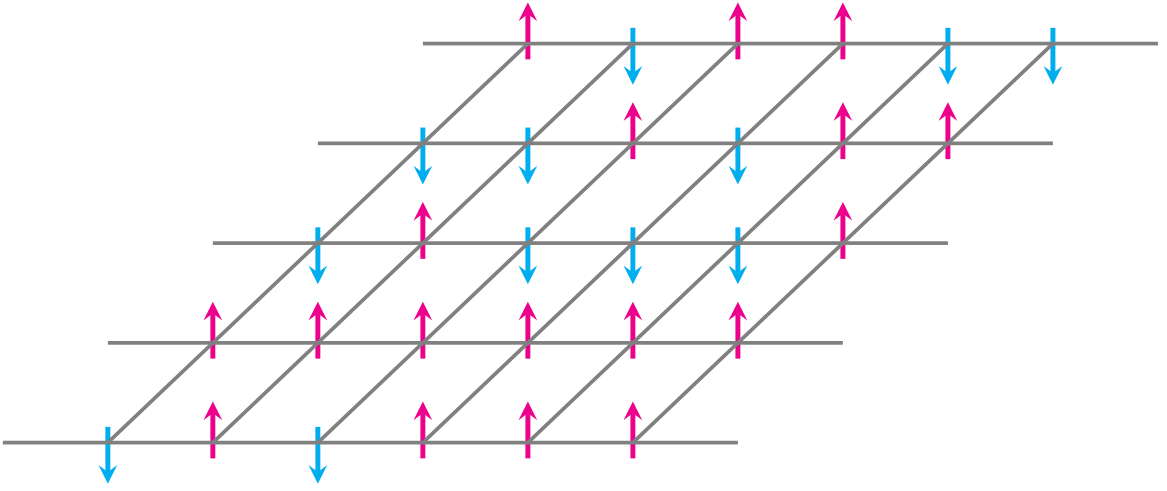
\includegraphics[width=0.7\textwidth]{fotos/2D_ising_model_on_lattice.svg.png}
    \caption{Ejemplo de un segmento de red del modelo de Ising bidimensional. \href{https://es.wikipedia.org/wiki/Modelo_de_Ising}{\textit{\underline{Fuente}}.} }
    \label{fig:ising-red}
\end{figure}
En general, el hamiltoniano de un sistema de este tipo es
\[
\mathcal{H} = -J\sum_{\langle i,j \rangle} s_i s_j - H\sum_i s_i,
\]
donde $s_i=\pm1$ es la variable de espín situada en el nodo $i$ de la red, $J$ es la constante de acoplamiento que relaciona la interacción entre espines con la energía y $H$ es un campo magnético externo uniforme acoplado a cada espín. Las dos sumas se extienden, respectivamente, a los pares de espines primeros vecinos de cada nodo y a todos los espines de la red.

Si $J>0$, el estado de mínima energía del hamiltoniano corresponde a un alineamiento de todos los espines, por lo que se trata de un material ferromagnético. Si en su lugar $J<0$, el estado de mínima energía corresponde a alineamientos en la misma dirección pero sentidos contrarios, dando lugar al antiferromagnetismo. En este trabajo se va a tratar el modelo de Ising en ausencia de campo magnético, por lo que $H=0$ y el hamiltoniano del sistema se simplifica a la interacción magnética entre espines, $\mathcal{H} = -J\sum_{\langle i,j \rangle} s_i s_j$, restringida ya a primeros vecinos.

El parámetro de orden natural para esta transición es la magnetización por espín, $m = \frac{1}{N}\sum_i s_i$, donde $N=L^2$ es el número total de espines de la red. En el límite termodinámico, $m=0$ a temperaturas mayores a $T_c$ y $m\neq 0$ por debajo, indicando el paso del estado paramagnético al ferromagnético. En un sistema finito, sin embargo, la simetría del hamiltoniano frente a la inversión global de todos los espines hace que el promedio de la magnetización por espín sea $\langle m \rangle = 0$ a cualquier temperatura, así que en las simulaciones se trabaja con $\langle |m| \rangle$ como estimador del parámetro de orden, que no sufre la misma simetría.

\section{Mecánica estadística}

En la colectividad canónica, el estado de equilibrio de un sistema en contacto con un baño térmico a temperatura $T$ queda determinado por la función de partición
\[
Z = \sum_{\{\sigma\}} e^{-\beta \mathcal{H}(\sigma)},
\]
con $\beta = \frac{1}{k_B T}$ y donde la suma se extiende a todos los posibles estados compatibles con el macroestado observado. Esta función contiene toda la información del sistema. Calcularla, ya sea de manera analítica o numérica, es equivalente a resolver el sistema. Esto permite obtener otras cantidades como la energía libre, la capacidad calorífica o la magnetización por partícula.

A partir de $Z$ se define la energía libre $F = -k_B T \ln Z$, de la que se derivan el resto de magnitudes termodinámicas. La energía media del sistema es
\[
\langle E \rangle = -\frac{\partial \ln Z}{\partial \beta},
\]
y la capacidad calorífica por partícula se obtiene derivando respecto a la temperatura,
\begin{equation} \label{eq:Cv}
    c = \frac{1}{N}\frac{\partial \langle E \rangle}{\partial T} = \frac{1}{N k_B T^2}\left(\langle E^2 \rangle - \langle E \rangle^2\right),
\end{equation}
expresión que relaciona $c$ con las fluctuaciones de la energía. De forma análoga, la susceptibilidad magnética por espín se relaciona con las fluctuaciones de la magnetización,
\[
\chi = \frac{1}{N k_B T}\left(\langle M^2 \rangle - \langle M \rangle^2\right),
\]
con $M = \sum_i s_i$ la magnetización total. Estas dos expresiones son usadas para calcular $c$ y $\chi$ a partir de los promedios medidos sobre las series temporales generadas en las simulaciones.

Otras dos cantidades usadas en este estudio son el cumulante de Binder y la longitud de correlación. El cumulante de Binder de cuarto orden se define como
\[
U_4 = 1 - \frac{\langle m^4 \rangle}{3\langle m^2 \rangle^2},
\]
y es una cantidad adimensional que en el límite termodinámico toma, justo en $T_c$, un valor universal que depende solo de la dimensionalidad y la simetría del sistema. Esto permite utilizarlo como una herramienta muy conveniente para localizar la temperatura crítica usando un sistema finito, como se explica en la sección de escalado de tamaño finito.

La longitud de correlación $\xi_L$ mide la distancia típica a la que están correlacionadas las fluctuaciones de espín, y se obtiene a partir de la función de correlación espín-espín $g(r) = \langle s_0 s_r \rangle - \langle s_0 \rangle \langle s_r \rangle$, que lejos de $T_c$ decae de forma aproximadamente exponencial, $g(r) \sim e^{-r/\xi_L}$, para $r$ grande. En una red finita con condiciones de contorno periódicas resulta más práctico trabajar con la llamada longitud de correlación de segundo momento \citep{Cooper1982, Newman1999}. Esta se construye a partir del factor de estructura, definido como la transformada de Fourier de la función de correlación,
\begin{equation} \label{eq:structure_factor}
    \chi(\mathbf{k}) = \frac{1}{N}\left\langle \left| \sum_j s_j\,
    e^{i\mathbf{k}\cdot\mathbf{r}_j} \right|^2 \right\rangle,
\end{equation}
donde $\mathbf{r}_j$ es la posición del espín $j$. Evaluándolo en el vector de
onda nulo y en el menor vector de onda no nulo compatible con la red, $k_{\min} = 2\pi/L$, la longitud de correlación de segundo momento se obtiene tras un desarrollo a segundo orden en el momento de la red y despejando \citep{Cooper1982},
\begin{equation} \label{eq:xi_def}
    \xi_L = \frac{1}{2\sin(\pi/L)}\sqrt{\frac{\chi(0)}{\chi(k_{\min})} - 1}.
\end{equation}
La ventaja de esta definición es que puede ser fácilmente calculada a partir de las mismas configuraciones de espín generadas para la medida del resto de observables y no requiere un cálculo explícito de $g(r)$ para cada distancia $r$.

Por último, queda por explicar cómo se calculan los valores esperados $\langle O \rangle$
que aparecen en todas las fórmulas anteriores. Estos son promedios sobre la colectividad
canónica, es decir, promedios fásicos pesados por el factor de Boltzmann,
\[
\langle O \rangle = \frac{1}{Z}\sum_{\{\sigma\}} O(\sigma)\,e^{-\beta\mathcal{H}(\sigma)},
\]
y no promedios temporales sobre una evolución dinámica del sistema. Como sumar sobre los
$2^N$ microestados es inviable, no evaluamos esta suma directamente, sino que recurrimos al muestreo por importancia: el algoritmo de Montecarlo genera una sucesión de configuraciones $\sigma_1,\dots,\sigma_M$ que, una vez alcanzado el equilibrio, están distribuidas según la propia distribución de Boltzmann; el índice que las ordena no es un tiempo físico, sino el número de pasos de Montecarlo. Para que esto sea válido basta con que la cadena de Markov sea ergódica, es decir, cualquier configuración es alcanzable desde cualquier otra, y satisfaga el balance detallado, condiciones que se imponen sobre los tres algoritmos más adelante (sección~\ref{sec:montecarlo}). Bajo ellas, se garantiza que el promedio aritmético sobre las configuraciones generadas converge al promedio fásico
buscado,
\[
\langle O \rangle \approx \frac{1}{M}\sum_{t=1}^{M} O(\sigma_t),
\]
donde $\sigma_t = \{s_i\}_t$ es la configuración completa de la red (el conjunto de los valores de todos los espines) en la $t$-ésima medida tras la termalización y $M$ es el número de medidas tomadas tras la termalización. Esta es la expresión que se aplica en la práctica para obtener $\langle E \rangle$, $\langle |m| \rangle$, $c$, $\chi$, $U_4$ y $\xi_L$ a partir de las simulaciones.


% =======================================================================================


\section{Transición de fase, temperatura crítica y exponentes críticos}

En el límite termodinámico, la transición de fase del modelo de Ising bidimensional ocurre exactamente en $T_c$ [ecuación \eqref{eq:Tc_onsager}], y alrededor de este punto las magnitudes termodinámicas dejan de ser funciones analíticas de la temperatura. En particular, la longitud de correlación diverge siguiendo una ley de potencias:
\[
\xi(T) \sim |T-T_c|^{-\nu},
\]
y el resto de cantidades exhiben un comportamiento similar, con diferentes exponentes: la magnetización se anula como $m \sim (T_c-T)^{\beta}$ para $T<T_c$, la susceptibilidad diverge como $\chi \sim |T-T_c|^{-\gamma}$, y la capacidad calorífica se comporta como $c \sim |T-T_c|^{-\alpha}$. En el caso del modelo de Ising bidimensional, esta última divergencia es solo logarítmica, lo que significa que $\alpha=0$.

Los exponentes $\nu$, $\beta$, $\gamma$ y $\alpha$ se llaman exponentes críticos, y su origen está en el hecho de que justo en $T_c$ la longitud de correlación se hace infinita y el sistema deja de tener una escala de longitud característica propia. De ahí, el comportamiento queda determinado únicamente por la dimensionalidad del sistema y la simetría del parámetro de orden, siendo independiente de los detalles microscópicos del hamiltoniano. Esto es lo que se conoce como universalidad: sistemas físicamente muy diferentes pueden presentar los mismos exponentes críticos siempre que tengan la misma dimensionalidad y simetría del parámetro de orden, lo que los junta en una misma \textit{clase de universalidad} \citep{Wilson1974}. El modelo de Ising bidimensional pertenece a su propia clase de universalidad, para la que los valores exactos de los exponentes son conocidos gracias a la solución analítica de Onsager y a las extensiones posteriores de esta \citep{Yang1952},
\[
\nu = 1,\quad \gamma = \frac{7}{4}.
\]
Estos son los valores de referencia que se utilizarán para comparar los resultados obtenidos a partir de la simulación con las predicciones teóricas.

\section{Escalado de tamaño finito} \label{sec:fss}

Las divergencias descritas en la sección anterior solo ocurren en el límite $L\to\infty$. En un sistema de tamaño finito, la longitud de correlación nunca puede superar el tamaño de la red, por lo que cerca de $T_c$ se satura en un valor del orden de $L$ en lugar de divergir, y todas las magnitudes termodinámicas son funciones suaves y continuas de la temperatura. La técnica de escalado de tamaño finito (\textit{finite-size scaling}, FSS) \citep{Fisher1972} parte de la suposición de que, cuando $\xi$ es del orden de $L$, la única razón relevante en el problema es $L/\xi$, y para cada cantidad debe existir una forma de escala que dependa de $L$ y de $T$ únicamente a través de la combinación $(T-T_c)L^{1/\nu}$. Para las magnitudes de interés en este trabajo, esto se traduce en
\[
\langle |m| \rangle (L,T) = L^{-\beta/\nu}\, f_m\!\left((T-T_c)L^{1/\nu}\right),
\]
\begin{equation} \label{eq:fss_chi2}
    \chi(L,T) = L^{\gamma/\nu}\, f_\chi\!\left((T-T_c)L^{1/\nu}\right),
\end{equation}
\begin{equation} \label{eq:fss_xi2}
    \xi_L(L,T) = L\, f_\xi\!\left((T-T_c)L^{1/\nu}\right)
\end{equation}
donde $f_m$, $f_\chi$ y $f_\xi$ son funciones universales dentro de cada clase de universalidad. Una consecuencia práctica de estas relaciones es que al representar $\langle|m|\rangle L^{\beta/\nu}$ o $\chi L^{-\gamma/\nu}$ frente a $(T-T_c)L^{1/\nu}$ para diferentes tamaños de red, todas las curvas deben colapsar en una única curva universal, siempre que los exponentes y $T_c$ utilizados sean los correctos. Esta es una de las formas más directas de verificar si los exponentes obtenidos son compatibles con los valores teóricos para la clase de universalidad del modelo de Ising bidimensional.

Otra consecuencia del tamaño finito en la simulación es que el máximo de magnitudes como $\chi$ o $c$ no se sitúa exactamente en $T_c$, sino en una temperatura pseudocrítica $T_c(L)$ que depende del tamaño de la red y que converge hacia $T_c$ a medida que $L$ crece, según \citep{Fisher1972}
\[
T_c(L) - T_c \sim L^{-1/\nu}.
\]
El cumulante de Binder $U_4=1-\frac{\langle m^4\rangle}{3\langle m^2\rangle^2}$ \citep{Binder1981} es muy útil en esta situación, ya que no tiene dimensiones, por lo que no tiene ningún factor adicional de $L$ en su forma de escala: $U_4(L,T) = f_U\!\left((T-T_c)L^{1/\nu}\right)$. Esta propiedad implica que en $T=T_c$ el valor de $U_4$ es independiente de $L$, y por tanto las curvas $U_4(T)$ obtenidas para distintos tamaños deben cruzarse todas en el mismo punto, y este punto puede utilizarse para determinar $T_c$ sin necesidad de ningún otro exponente.

\section{Tiempo de correlación} \label{sec:csd}

Conviene precisar primero qué se entiende aquí por tiempo. Una simulación de Montecarlo no reproduce la evolución dinámica real del sistema, sino que las configuraciones se obtienen aplicando una regla de actualización estocástica. Por tanto, no existe un tiempo físico, ya que el recorrido se está realizando sobre una serie de configuraciones del espacio fásico. Lo que se llama tiempo es sencillamente el índice que ordena la sucesión de configuraciones, medido en pasos Montecarlo (sección~\ref{sec:pasomc}). Es una propiedad discreta, adimensional e intrínseca al algoritmo. En lo que sigue, se entiende por tanto cualquier escala temporal en pasos Montecarlo.

Estos algoritmos generan una sucesión de configuraciones $\sigma_1,\sigma_2,\dots,\sigma_M$ que no son estadísticamente independientes entre sí, ya que cada una se obtiene a partir de la anterior mediante pequeñas modificaciones. La correlación entre configuraciones consecutivas se mide a partir de la función de autocorrelación para una cantidad $O$ \citep{LandauBinder},
\[
C_O(t) = \langle O(t_0)\, O(t_0+t) \rangle - \langle O \rangle^2,
\]
que típicamente decae de forma exponencial, $C_O(t) \sim e^{-t/\tau_O}$, donde $\tau_O$ es el tiempo de correlación asociado a $O$. Cuanto mayor es $\tau_O$, más pasos de Montecarlo hay que esperar entre dos medidas para que puedan considerarse independientes, y por tanto mayor es el error estadístico real de una media calculada con un número dado de configuraciones: el número efectivo de medidas independientes es del orden de $M/(2\tau_O)$ en lugar de $M$.

Cerca de la temperatura crítica, donde $\xi$ crece, el tiempo de correlación también crece. Esto se conoce como ralentización crítica (\textit{critical slowing down}), y está descrito por el exponente dinámico $z$ \citep{HohenbergHalperin1977},
\[
\tau \sim \xi^{z} \sim L^{z}.
\]
A diferencia de los exponentes estáticos $\nu$, $\beta$ o $\gamma$, el exponente $z$ no depende solo de la clase de universalidad del sistema, sino también del algoritmo empleado para generar la dinámica. Los algoritmos de actualización local, como Metropolis o Glauber, tienen para el Ising 2D un exponente dinámico relativamente grande, $z \approx 2{,}17$, lo que hace que cerca de $T_c$ el número de pasos necesarios para obtener medidas independientes crezca muy rápidamente con $L$. Los algoritmos de tipo \textit{cúmulo} \citep{SwendsenWang1987}, como el de Wolff, fueron ideados para evitar o mitigar el ralentizamiento crítico y presentan valores de $z$ cercanos a cero para el modelo de Ising bidimensional. Esta diferencia en el comportamiento de $\tau$ con $L$ cerca del punto crítico es uno de los aspectos principales que se comparan en este trabajo entre los tres algoritmos implementados.

En la práctica, los tiempos de correlación se calculan a partir de las series temporales generadas por la simulación. Para una magnitud $O$, se calcula la función de autocorrelación normalizada
\[
\rho_O(t) = \frac{C_O(t)}{C_O(0)},
\]
que decae de $1$ a $0$ a medida que $t$ aumenta. A partir de ella se define el tiempo de autocorrelación integrado,
\begin{equation} \label{eq:tau_int}
   \tau_{\text{int},O} = \frac{1}{2} + \sum_{t=1}^{\infty} \rho_O(t), 
\end{equation}
que es la cantidad que determina el error estadístico real de la media $\langle O \rangle$: si las $M$ medidas no fueran independientes sino que estuvieran correlacionadas con tiempo $\tau_{\text{int},O}$, la varianza del estimador de la media sería \citep{Wolff2004}
\[
\sigma^2(\langle O \rangle) \approx \frac{2\tau_{\text{int},O}}{M}\,\text{Var}(O).
\]
En la suma que define $\tau_{\text{int},O}$ no se puede llegar hasta infinito con datos finitos, ya que para $t$ grande $\rho_O(t)$ se vuelve ruidosa. En la práctica se trunca la suma en algún tiempo $t^*$ a partir del cual $\rho_O(t)$ ha decaído suficientemente, lo que requiere un cierto cuidado para no subestimar $\tau_{\text{int},O}$ truncando demasiado pronto ni sobreestimarlo acumulando ruido al truncar demasiado tarde.